\section{基于$L_1$范数主成分分析的高维因子模型估计}\label{chapter2}

\subsection{因子模型及其估计}
因子模型是主成分分析的推广和发展,它也是多元统计中广泛使用的一种降维方法。
因子模型研究相关矩阵或者协方差矩阵的内部依赖关系,它将多个变量综合为少数几个因子,
以再现原始变量和因子之间的关系。

\subsubsection{正交因子模型}

设$\bm{X} = (X_1, X_2, ..., X_p)^T$是可观测的随机向量,$\mathbb{E}\bm{X} = \bm{\mu}$,
$\mathbb{D}(\bm{X}) = \bm{\Sigma}$,设$\bm{f} = (f_1, f_2, ..., f_m)^T\\ (m <p)$为不可观测的随机向量,且
$\mathbb{E}\bm{f} = 0$,$\mathbb{D}(\bm{f}) = \bm{I}_m$(即$\bm{f}$的各分量方差为1,且互不相关)。最后,设
$\bm{e} = (e_1, e_2, ..., e_p)^T$和$\bm{f}$互不相关,并且
$$
    \mathbb{E}(\bm{e}) = \bm{0}\mbox{,}\mathbb{D}(\bm{e}) = diag({\sigma _1}^2, ..., {\sigma _p}^2)
    \mbox{为对角矩阵。}
$$
假设随机向量$\bm{X}$满足以下模型:
\begin{equation} \label{orth-factor}
\left\{
\begin{array}{clr}
    X_1 - \mu_1 = a_{11}f_1 + a_{12}f_2 + ... + a_{1m}f_m + e_1, \\
    X_2 - \mu_2 = a_{21}f_1 + a_{22}f_2 + ... + a_{2m}f_m + e_2, \\
    ... \\
    X_p - \mu_p = a_{p1}f_1 + a_{p2}f_2 + ... + a_{pm}f_m + e_p,
\end{array}
\right.
\end{equation}
我们称该模型为正交因子模型,矩阵表示为:
\begin{equation}
    \bm{X} = \bm{\mu} + \bm{A}\bm{f} + \bm{e}
\end{equation}
其中$f_1, f_2, ..., f_m$称为$\bm{X}$的公共因子;$e_1, e_2, ..., e_p$称为$\bm{X}$
的特殊因子。公共因子一般对$\bm{X}$的每一个分量都起作用,而$e_i$一般仅仅对$X_i$起作用。
并且各个特殊因子之间以及特殊因子和所有公共因子之间都是不相关的。
其中$\bm{A} = (a_{ij})_{p \times m}$是待估计的系数矩阵,称为因子载荷矩阵。
$a_{ij}$称为第$i$个变量在第$j$个因子上的载荷,它反映了第$i$个变量在第$j$个因子上的相对重要性。

对于正交因子模型,
在因子载荷矩阵$\bm{A}$中,我们计算各列的平方和,记为$q_j^2$,即
\begin{equation}
    q_j^2 = \sum_{i=1}^p a_{ij}^2 (j = 1, 2, ..., m)
\end{equation}
$q_j^2$表示第$j$个公共因子$f_j$对$\bm{X}$的所有分量的总影响,称为公共因子$f_j$对$\bm{X}$的
方差贡献。因此如果我们列出$\bm{A}$的所有列平方和,按照方差贡献大小就可以选出最有影响的公共因子。
因此因子分析的关键步骤就是估计出因子载荷矩阵。

对于正交因子模型可以通过主成分法、主因子法和极大似然法来估计因子载荷矩阵。不可观测的公共因子有时候也需要进行估计,
例如用来诊断因子模型或者作为进一步分析的原始数据,这就需要我们给出因子得分,一般在得出了因子载荷矩阵之后,
对于因子得分,可以通过加权最小二乘法(巴特莱因子得分)或者通过回归法(汤普森因子得分)进行估计。

但是对于动态因子模型和近似动态因子模型,因为不满足正交因子模型的一些关键模型假设,因此需要不同的估计手段。
\subsubsection{动态因子模型}

令$\bm{X}_t = (\bm{X}_{1t},\bm{X}_{2t}, ..., \bm{X}_{pt})^T$为一组宏观经济变量在$t$时刻的水平,并且$\bm{X}_t$可以表达为如下形式:
\begin{equation}
    \bm{X}_t = \lambda(L)\bm{f_t} + e_t
\end{equation}
其中,$\bm{f}_t$ 为$q\time 1$ 维的动态因子向量,$\lambda(L)$为由$s$阶滞后多项式算子组成的$p \times q$矩阵。
动态因子模型通常假设动态因子向量服从某一个向量随机过程。即动态因子模型
不仅允许观测变量受因子滞后项的影响,而且也允许因子本身具有独立的动态演化过程。

动态因子模型的提出者Geweke和Sargent等人都是使用频域方法估计模型,这种方法不能够直接估计出动态因子$\bm{f}_t$,
因此也就不能将因子作为预测或者扩展模型等用途。使得动态因子模型的应用收到限制。

\subsubsection{近似因子模型}
Chamberlain 和 Rothschild放弃 异质性部分的协方差矩阵为对角阵 的假定,允许异质性部分存在一定程度的截面相关, 
模型假设允许$f_t$的各个分量$f_1, f_2, ..., f_m$具有相依性,$e_1, e_2, ..., e_p$可以不独立,
并且允许$f_t$,$e_t$具有时间序列相依性。从而将模型扩展为了为动态近似因子模型,也简称为近似因子模型。

由于动态近似因子模型估计困难,因此在预测中,往往使用模型的静态形式:
\begin{equation}\label{s-fac}
X_t = AF_t + e_t
\end{equation}
式\eqref{s-fac}中,$F_t$是$m$维向量,称为静态因子,即$F_t$仅在当期影响$X_t$(因为$F_t$包括了动态因子$f_t$的当期项和
滞后项),它本身可以不具有经济学含义。$A$是因子载荷矩阵。本文采用\eqref{s-fac}中的模型进行宏观经济指标的预测。

对于静态形式的估计,Stock和Watson于1989年最早提出了一种方法\cite{stock1989new}:这种方法采用
Kalman 滤波构造似然 函数,并采用极大似然方法来估计参数。
这种方法的 优点是: 在误差项服从正态分布的假定下,能够得到 因子的有效估计量。
然而,由于在估计参数过程中 会应用到非线性数值优化算法,而待估参数的个数与变量维数$p$成比例,
限于当时的计算能力,这种方法只能用于处理低维的精确动态因子模型。

针对维数很高的宏观经济变量,Stock和Watson于2002年给出了一种非参数的方法\cite{stock2002forecasting},并且得到广泛使用。
这种方法使用主成分分析法进行估计,对\eqref{s-fac},因子载荷矩阵$\bm{A}$的估计量$\hat{\bm{A}}$即为
$\bm{X}_t$的样本协方差矩阵
\begin{equation}\label{fac-pro}
\hat{\bm{\Sigma}}_{\bm{X}} = \frac1{n}\sum_{t=1}^n\bm{X_t}\bm{X_t}^T
\end{equation}
的前
$r$个最大特征值所对应的特征向量组成的$p\times r$维矩阵,静态因子的主成分估计量为:
\begin{equation}\label{factor}
\hat{\bm{F}} = \hat{\bm{A}}\bm{X}_t 
\end{equation}

主成分估计量具有一系列良好的性质。例如, 在$p \rightarrow \infty$, $n \rightarrow \infty$ 且 $p^2 / n \rightarrow \infty$
的条件下,主成分估计量$\hat{\bm{F}}_t$是因子空间的一致估计量,且在随后的建模 过程中可以当作观测到的数据。

\subsection{$L_2$范数主成分分析}
在许多领域的数据分析中,常会遇到输入变量维数很高的情况,为了方便对建立模型或处理数据,
常常需要通过某些方法将输入变量个数减少。人们希望同时同时做到减少输入变量的个数、简化问题复杂度的同时
尽量不损失原始数据的信息,因此直接舍弃变量的做法一般是不可取的。

比较合适的解决办法是通过某种手段,将高维变量组成的数据集映射到低维,并且尽量保持数据集的信息量。这种方法称为
数据降维。降维后的数据既包含原数据绝大部分的信息,同时又具备容易分析和处理的特点。

主成分分析(principal component analaysis, PCA)就是一种十分流行的数据降维方法,它已经在信号处理、机器学习等众多领域
得到了广泛应用。在经济学、心理学等社会科学领域的一个重要应用就是对因子模型进行估计。

通常,一个数据集总是由若干随机变量的若干观测组成。主成分分析的目标就是将原始数据集进行降维,
将这些观测投射到一个低维空间中。这样的投射有无数种,主成分分析希望找到这样一种投射,可以使得
数据在低维空间的投影拥有最大的方差,因为在统计学上,方差反映了样本数据中包含的信息量。

如果使用规范的数学表述,$L_2$主成分估计分析问题可以表述为
\begin{equation}\label{pca-l2-p1}
P_1: \ \hat{\bm{A}}_{p\times m}, \hat{\bm{F}}_{m\times n} = \underset{\bm{A},\bm{F}}{\operatorname{arg\ min} } 
\|\bm{X} - \bm{A}\bm{F}\|_{L_2}
 = \underset{\bm{A}, \bm{F}}{\operatorname{arg\ min}} \sum_{i=1}^p \sum_{j=1}^m (x_{ij} - a_i^Tf_i)^2 .
\end{equation}
其中$\bm{X}$为$p \times n$的高维数据矩阵,$\bm{A}$的列构成了$\bm{X}$的$m$维线性子空间的基,这个子空间也称为特征空间。
$\bm{F}$为一系数矩阵,给出了$\bm{X}$各列元素在特征空间中的坐标,根据矩阵投影理论,在给定$\bm{A}$的条件下,
$\bm{F} = \bm{A}^T \bm{X}$。
问题$P_1$可以解释为,需要找到一个合适的投射矩阵,使得数据在低维的投影上升回高维空间后和原矩阵各元素的误差平方和最小。

对于问题$P_1$常用奇异值分解法求解。同样地我们也可考虑其对偶问题$P_2$,
\begin{equation}\label{pca-l2-p2}
P_2: \ \hat{\bm{A}} = \underset{\bm{A}}{\operatorname{arg\ max}} \| \bm{A}^T \bm{X}\|_{L_2}, \text{其中}\ \bm{A}^T
\bm{A} = \bm{I}_m
\end{equation}

问题$P_2$可以理解为,需要找到一个合适的投射矩阵,使得数据在低维空间的投影有最大的方差。在统计学上,数据的方差反映了数据中信息的多少,
因此在特征空间中选取方差最大的方向作为主成分是很恰当的。
因此常用特征值分解的方法求解$P_2$,原因是原始数据协方差矩阵的某一特征值就是该特征值对应特征向量的方差,
因此我们只要对原始数据的协方差矩阵进行特征值分解,找出最大的一些特征值,它们对应的特征向量就可以作为主成分了。
通常用主成分方向上的方差的和占据总方差的比例来衡量主成分包含原始数据信息量的多少。

对于\eqref{fac-pro},下面给出使用特征值分解进行主成分分析的步骤:
记矩阵$\bm{X}_{p\times n}$为$p$维宏观经济变量$\bm{X}_t$在$t_1, ..., t_n$的$n$次观测,

1. 将$\bm{X}$进行中心化;

2. 计算样本协方差矩阵$\frac1{n}\bm{X}\bm{X}^T_{p\times p}$;

3. 对样本协方差矩阵特征值分解,并从小到大排列这些特征值;

4. 因子载荷矩阵估计量$\hat{\bm{A}}_{p\times m} (m < p)$为前$m$个特征值对应的特征向量组成的矩阵。

不难看出,主成分分析法进行估计的关键计算步骤是对样本协方差矩阵的特征值分解。
而奇异值分解解决将矩阵$\bm{A}$分解成正交矩阵$\bm{U}$和对角矩阵$\bm{\Sigma}$和另一正交矩阵$\bm{V}^T$的问题,即
$$
    \bm{A}_{m \times n} = \bm{U}_{m \times m}\bm{\Sigma}_{m \times n}\bm{V}_{n \times n}^T
$$

奇异值分解求解的关键就是得到奇异值,而后者是$\bm{A}^T\bm{A}$的特征值的平方根,即奇异值分解的关键计算步骤是对
$\bm{A}^T\bm{A}$进行特征值分解。这里假设我们取$\bm{A} = {\bm{X}^T}/{\sqrt{m}}$,不难看出和特征值分解法等价。

为了方便起见,下面我们把求解$P_1$和$P_2$统称为$L_2$范数主成分分析。

\subsection{$L_1$范数主成分分析}

$L_2$范数主成分分析具有
所有的$L_2$范数优化方法普遍的缺陷,那就是对离群值十分敏感。并且特征分解和奇异值分解都不能直接处理具有缺失值的数据,
因此对于缺失数据必须进行插补。

然而由于各种原因,高维宏观经济数据中往往具有大量的缺失值和离群值,这就给因子模型的估计带来很多的麻烦,
从而进一步使用因子的估计量进行预测可能会变得不够准确。

将$P_1$中的目标函数更换为使用$L_1$范数,可得
\begin{equation}\label{p3}
    P_3: \ 
\hat{\bm{A}}_{p\times m}, \hat{\bm{F}}_{m\times n} = \underset{\bm{A},\bm{F}}{\operatorname{arg\ min} } \|\bm X - \bm{A}\bm{F}\|_{L_1}
= \underset{\bm{A}, \bm{F}}{\operatorname{arg\ min}} \sum_{i=1}^p \sum_{j=1}^m |x_{ij} - \bm a_i^T \bm f_i| 
\end{equation}

若同样假设$\bm{A}_{p\times m}$为$\bm{X}$子空间的基组成的矩阵,即问题$P_1$就转化为问题$P_3$。
同样地,改变问题$P_2$,若我们想要寻找一个投射使得数据在低维的投影有最大的$L_1$范数,这就得到问题$P_4$。
我们把$P_3$和$P_4$称为$L_1$范数主成分分析,注意到这里$P_3$和$P_4$不再是对偶问题。
所以求解$L_1$范数主成分分析,常常是解决这两个问题其中之一。

\subsubsection{$L_1$范数简介}
在数学上范数主要包括向量范数和矩阵范数,向量范数描述了向量在空间中的大小,而矩阵范数描述了矩阵引起变化的大小。
首先介绍向量$L_p$范数,$L_p$范数是如下定义的一组范数
\begin{equation}
    L_p = \| \bm x\|_{L_p} = (\sum_{i=1}^n x_i)^{\frac{1}{p}}, \bm x= (x_1, ..., x_n)
\end{equation}
根据$p$的变化,$L_p$范数也会发生变化。

常用的向量范数主要有三种,分别是$L_0$范数、$L_1$范数和$L_2$范数。
其中$$L_0 = \| \bm x\|_{L_0} = \sum_{i=1}^n\mathbb I[x_i \neq 0]$$即向量中非0元素个数。
而$$L_1 = \| \bm x\|_{L_1} = \sum_{i=1}^n|x_i|$$而$$L_2 = \|\bm x \|_{L_1} = (\sum_{i=1}^n x_i^2)^{\frac1{2}}$$
其中$L_2$范数是最常用的范数。对于矩阵来说其$L_1$范数就是所有元素的绝对值合,$L_2$范数就是所有元素的平方之合。

$L_1$范数在统计学中主要有两种用途。一种是作为稳健手段,因为在优化问题中,作为目标函数的$L_2$范数对于离群值具有放大作用,
而作为目标函数的$L_1$范数则更具稳健性;另一种应用是给模型添加稀疏约束,在线性模型中也称为$L_1$正则化,
在求解某个最优向量的场合,如果同时最小化该向量的$L_1$范数,
那么就可以得到具有稀疏性的解(即解的$L_0$范数很小),这是由于$L_1$范数和$L_0$范数的天然联系造成的。


\subsubsection{求解$L_1$范数主成分分析的交替凸优化算法}

一种经典的方法是使用交替凸优化算法\cite{ke2005robust}求解$P_3$。该算法的思想是,当我们
面临一个两变量的优化问题,而该问题不是凸优化问题因此无法求其最优解时,可以采用迭代的方法,
每一步将其中一个未知变量的值看作是常数(使用该变量上次迭代的取值),来求解另一个
未知量。

我们注意到\eqref{p3}中定义的问题不是一个凸优化问题。但是一旦矩阵$\bm{A}$或者$\bm{F}$固定为常数,那么该问题就成为了一个凸优化问题,
可以找到全局最优解。给出一个

\begin{equation}\label{pro1}
\bm F^{t} = \underset{\bm F}{\operatorname{arg\ min}} \|\bm{X} - \bm{A}^{t-1}\bm{F} \|_{L_1} 
\end{equation}

\begin{equation}\label{pro2}
\bm{A}^{t} = \underset{\bm{A}}{\operatorname{arg\ min}} \|\bm X - \bm{A}\bm F^{t}\|_{L_1} 
\end{equation}
我们改写式\eqref{pro1}中的目标函数,
\begin{equation}\label{loss-a}
E(\bm{F}) = \|\bm{X} - \bm{A}^{t-1}\bm{F} \|_{L_1} = \sum_{j=1}^{n}|\bm{x}_j - \bm{A}^{t-1}\bm{f}_j| 
\end{equation}
其中$x_j$是矩阵$X$的第j列,$f_j$是$\bm{F}$的第j列。于是式\eqref{pro1}问题可以分解为$n$个独立的子优化问题,
求解相应的$\bm{f}_j$:
\begin{equation}\label{subpro}
    \bm{f}_j = \underset{\bm{\theta}}{\operatorname{arg\ min}} |\bm{A}^{t-1}\bm{\theta} - \bm{x}_j|
\end{equation}
同样地,\eqref{pro2}可以转化为下面的$p$个独立的子优化问题,
\begin{equation}\label{subproabs}
    \bm{a}_i^T = \underset{\bm{\theta}}{\operatorname{arg\ min}} |\bm{x}_i^T - \bm{F}^T\bm{\theta}|
\end{equation}
其中$\bm{a}_i$为$\bm{A}$的第$i$行,而$\bm{x}_i$为$\bm{X}$的第$i$行。

问题\eqref{subpro}和\eqref{subproabs},都可以采用线性规划问题求解。可以看出,在每次迭代我们都需要解决多个
线性规划的问题,而多变量多约束的线性规划求解速度很慢,这决定了交替凸优化算法的计算开销是比较大的。
事实上,限制$L_1$主成分分析的一个
重要原因就是它的计算复杂度太高。在本文后续内容中,将会进一步讨论相关步骤的计算优化问题,
尝试对交替凸优化算法做出改进。

使用特征值分解法或奇异值分解法时我们需要对矩阵$\bm{X}$进行缺失值插补,然后才能进行计算。
在$L_1$主成分分析中我们不需要进行缺失值插补,在式中,遇到$x_j$具有缺失值的场合,我们直接舍弃相应的
约束条件即可。
我们改写\eqref{loss-a},
$$E(\bm F) = \sum_{i=1}^d \sum_{j=1}^n |x_{ij} - \bm a_i^T\bm f_j|$$
如果某个项$x_{ij}$缺失,我们直接舍弃目标函数中的对应累加项,在上述算法中对应的做法就是直接删除\eqref{subpro}的一个约束条件。

需要注意的是,交替凸优化算法只能保证在每一步求得当前最优解,并不能保证最后得到$P_3$的全局最优解。

\subsubsection{算法步骤}
我们已经发现可以通过交替优化算法求解$L_1$范数主成分分析,下面我们更加详细地讨论该算法一些细节和具体实现步骤。

在算法开始时,首先我们需要给$\bm{A}$一个初始值$\bm{A}^{(0)}$。对于$\bm{A}$可以采用简单随机数进行初始化,这里我们
为了加快收敛速度,可以使用经过缺失值插补(这里我们使用均值插补)后通过PCA算法进行得到的因子载荷矩阵作为$\bm{A}^{(0)}$。
在本章后续小结的实验中我们可以发现,在含有大量缺失值和离群值的条件下,两种不同的初始化方法最终结果差异并不大。

因为目标函数$E(\bm{A}, F) = \|X - \bm{A}\bm{F}\|_{L_1}$在每一个交替的优化步骤中都递减,并且$E(\bm{A},F)$具有下界($\geq 0$)。
因此交替优化算法一定收敛。因此我们可以设定一个收敛域值来停止迭代,这里我们设置终止条件:
    $$ \theta(a_i^{(t)}, a_i^{(t-1)}) <  \alpha $$
这里$\theta(a, b)$表示向量$a$和$b$的夹角;其中$a_i$是$\bm{A}$或者$F$的第i列;$\alpha$是一个很小的正数。

算法3.1给出了算法具体步骤,其中归一化步骤是为了计算过程中保持数值的稳定性。在最终求解得到$\hat {\bm{A}}$后,我们可以对其
进行QR分解来得到主成分。

\begin{table}[H]%%%%%%开始表格
    \centering%把表居中
    \begin{tabular}{{p{0.9\columnwidth}}}%三个c代表该表一共三列,内容全部居中
    
    \toprule%第一道横线 表头
    算法3.1:交替凸优化求解$L_1$主成分分析 (ACP, Alternate Convex Programming) \\
    \midrule%第二道横线 符号+解释+单位 中间用&隔开
    1.初始化:给出$\bm{A}$,$\Sigma$的初始值$\bm{A}^{(0)}$,$\Sigma^{(0)} = I$,(其中$\Sigma$为一对角矩阵,
    $I$为单位矩阵); \\

    2.交替凸优化:对于迭代次数$t = 1, ..., T$: \\
    $$ F^{(t)} = \underset{F}{\operatorname{arg\ min}} \|X - \bm{A}^{(t-1)}\Sigma^{t-1}F^{T}\|_{L_1}$$ \\
    $$ \bm{A}^{(t)} = \underset{\bm{A}}{\operatorname{arg\ min}} \|X - \bm{A}\Sigma^{t-1}F^{Tt} \|_{L_1}$$ \\
    \begin{equation*}
        \text{归一化:}\left\{
                    \begin{array}{clr}
                    N_a = diag(\bm{A}^{(t)T}\bm{A}^{t})\\
                    N_f = diag(F^{Tt}F^{t})\\
                    F^{t} \leftarrow F^{t}N_f^{-1}\\
                    \bm{A}^{t}\leftarrow \bm{A}^{t}N_a^{-1}\\
                    \Sigma^{t} \leftarrow N_a\Sigma^{t-1}N_f\\
                    \end{array}
        \right.
    \end{equation*} \\

    3.输出结果:$\bm{A} \leftarrow \bm{A}^T\Sigma^{1/2}$,对$\bm{A}$进行QR分解取正交矩阵得到$\hat{\bm{A}}$;
    $\hat{\bm{F}} \leftarrow \hat{\bm{A}}^T\bm{X}$。 \\
    \bottomrule%第三道横线
    \end{tabular}
\end{table}%%%%%%结束表格

\subsection{稳健性实验}\label{lab-1}
为了检验$L_1$范数主成分分析在处理含有大量离群值和缺失值的数据时的稳健性,我们进行模拟实验,
来对比$L_2$范数主成分分析。

\subsubsection{数据准备}
为了进行模拟实验,我们首先需要随机产生一个高维低秩的矩阵来模拟高维宏观经济数据集。
我们产生一个$n$维方阵$M$,其中每一个随机元素均服从$[-100, 100]$的均分分布。然后我们对方阵$M$进行奇异值分解
,$M = U\Sigma V^{T}$。假设我们需要产生的低秩矩阵的秩为$r$,则$$X = U_{(:,1:r)}\Sigma_{(1:r,1:r)}V^T_{(:,1:r)}$$
即为我们得到的模拟高维低秩矩阵。

之后我们可以设置一定比例的缺失值和离群值,首先我们在矩阵的左下角剔除部分元素。在剩下的元素中,我们随机选取一部分
然后重新产生随机元素,每个元素服从$[-2000,2000]$上的均匀分布。图2.1展示了一个$30\times30$秩为3的
矩阵在模拟了缺失值和离群值后的情况。

\begin{figure}[H]
    \centering
    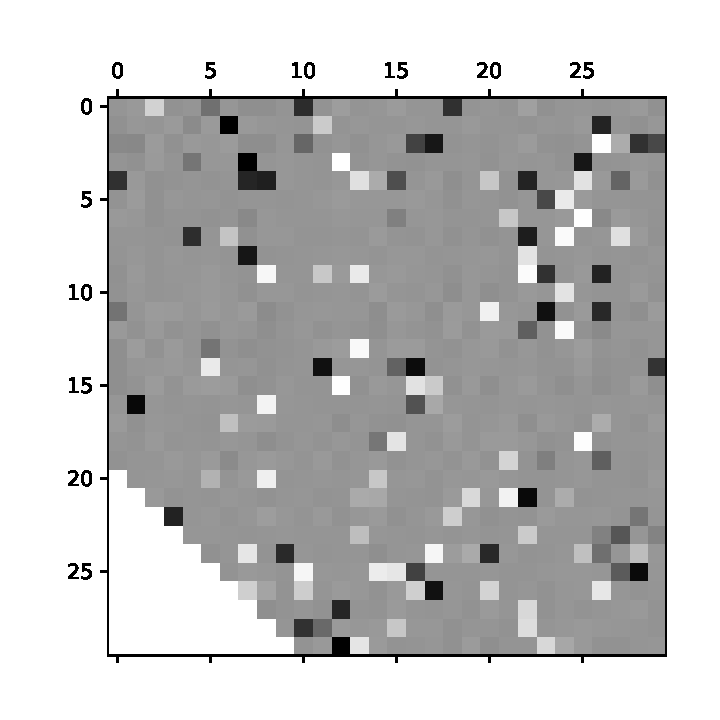
\includegraphics[width=.5\textwidth]{pics/chapter2/matrix.pdf}
    \caption{\small $30\times30$的模拟矩阵,左下角白色代表缺失值,图中灰度越深代表元素的绝对值越大,因此深黑色的点代表了离群值}
    \label{fig2.1}
\end{figure}

基于获得的高维低秩矩阵,我们主要比较以下算法:
对于$L_1$范数主成分分析,我们使用IRP算法。
对于$L_2$范数主成分分析,采用了下面三种算法:
1)奇异值分解,该算法需要进行缺失值插补,这里我们使用均值插补法。记作SVD;
2)基于IRP算法,但是更换损失函数为$L_2$范数,可以直接处理原始数据。记作IRP-L2;
3)一种基于迭代加权$L_2$范数的估计方法(Black和Rangarajan,1996),
通过将问题$P_1$损失函数加上随迭代变化的权重,可给$L_2$范数主成分分析带来一定的稳健性
,可以直接处理原始数据。记作IRLS(iteratively reweighted least squares)。

\subsubsection{实验结果}
令$\hat{\bm{X}} = \hat{\bm{A}}_{N \times M}\hat{\bm{F}}_{M \times N}$,我们比较因子残差
$\bm{E} = \hat{\bm{X}} -\bm{X}$。观察重构残差的平方的分布情况,
试验每一种算法作用在无干扰数据上和干扰后数据上的情况。

对于无干扰数据,每一种算法都具有很好的表现;
对于进行了缺失值和离群值模拟的数据,我们每组试验(给定$M$,$ N$)下均重复多次取平均值,图2.3给出了一个典型结果。
\begin{figure}[H]
    \centering
    \begin{minipage}[t]{0.48\textwidth}
    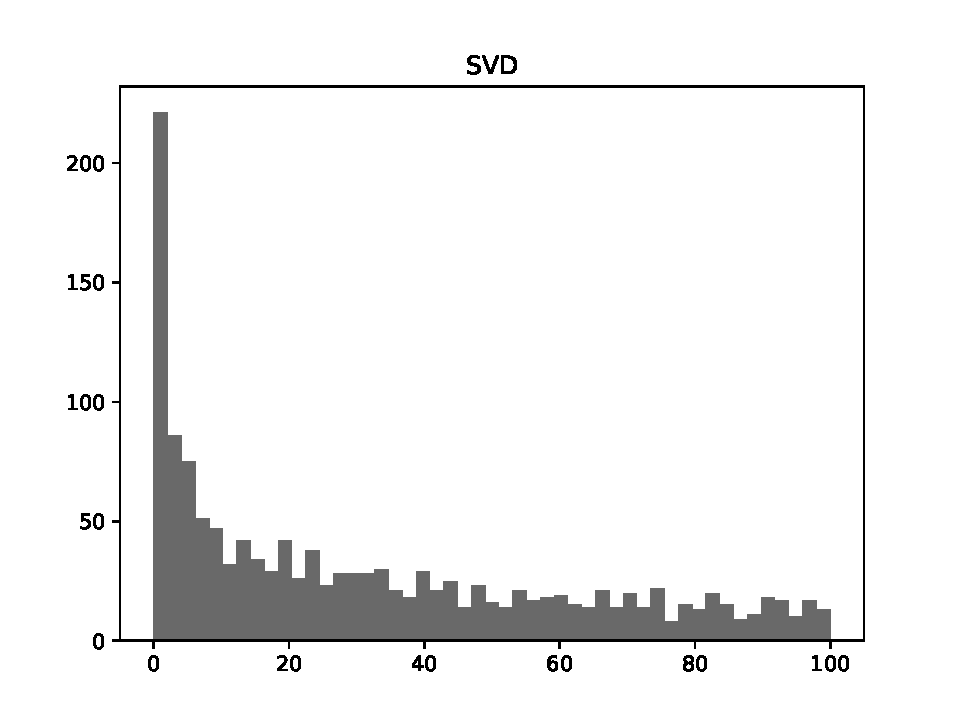
\includegraphics[width=8cm]{pics/lab1/svd.pdf}
    \end{minipage}
    \begin{minipage}[t]{0.48\textwidth}
    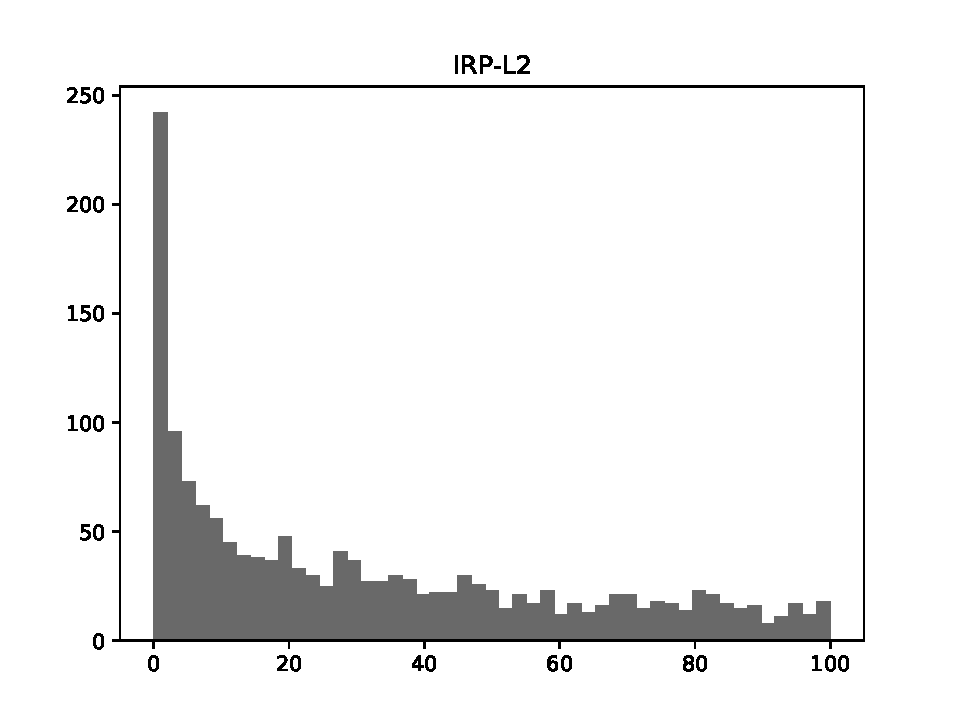
\includegraphics[width=8cm]{pics/lab1/IRP-L2.pdf}
    \end{minipage}
    \begin{minipage}[t]{0.48\textwidth}
    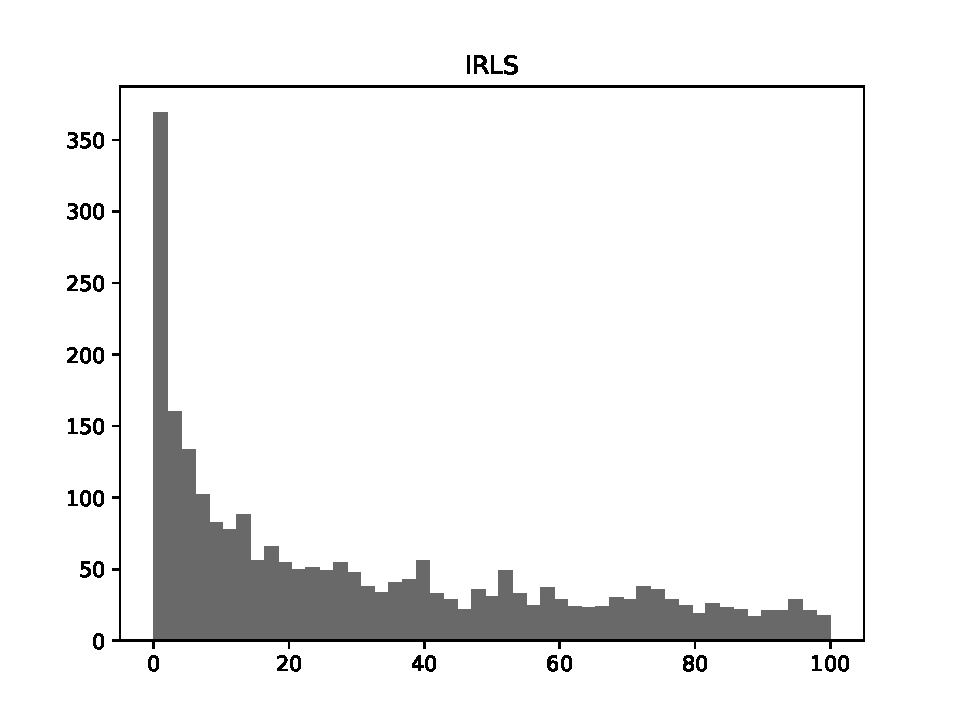
\includegraphics[width=8cm]{pics/lab1/IRLS.pdf}
    \end{minipage}
    \begin{minipage}[t]{0.48\textwidth}
    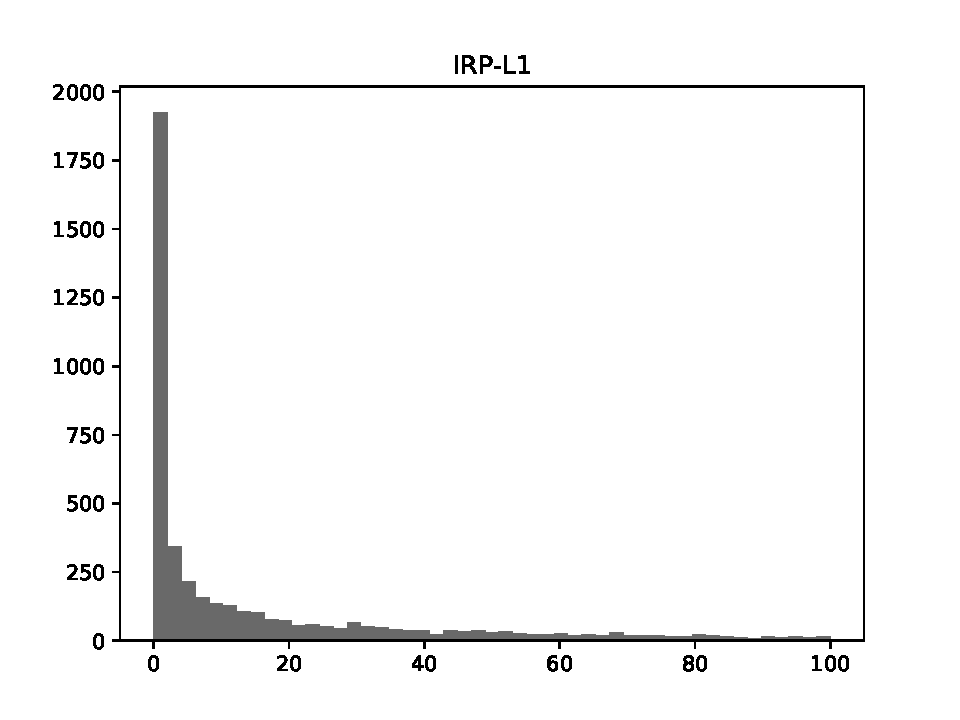
\includegraphics[width=8cm]{pics/lab1/IRP-L1.pdf}
    \end{minipage}
    \caption{\small 图示为取$N = 80, M=3$,缺失值和离群值比例均为$10\%$的情况下,多次实验中平均重构残差的平方的分布情况,横轴表示残差平方,
    纵轴表示频数。
    可以看出IRP-L1的重构残差表现最好。}
\end{figure}

实验表明,$L_1$范数主成分分析相比$L_2$主成分分析法和其他基于$L_2$范数优化的方法相比具有更好的稳健性,
特别适合于处理具有大量离群值的数据。

\subsection{基于国内主要月度宏观经济数据的实证研究}
上一节我们阐述了$L_1$范数主成分分析方法,本节我们进行基于国内主要月度宏观数据的实证研究,来探究
使用$L_1$范数主成分分析用来代替$L_2$范数主成分分析进行近似因子模型估计的可行性。

数据方面将选择高维的国内主要月度宏观经济数据,该数据集包含众多的经济指标,其中许多经济指标
具有重尾分布,即意味着包含较多的离群值。并且该数据集在时间序列上不完整,一些经济指标的观测值缺失。

本实证研究采用扩散指数模型进行经济预测\cite{stock2002macroeconomic},近年来该模型已经得到了广泛的应用。
该预测模型依赖近似因子模型的因子得分估计作为关键自变量,本次研究将对比$L_2$范数和$L_1$范数主成分分析
下不同的因子得分估计在宏观经济指标预测中的表现。最后,将结合实证结果对$L_1$范数主成分分析在
本场合的应用提出一些建议。

\subsubsection{扩散指数模型}
令$y_t$为待预测经济变量$y$在时间$t$的水平,$\bm{X}_t$为
$p$维随机向量,假设$(X_t,y_t)$服从近似因子模型并且$\bm{X}_t$和$y_t$具有相依性,
若$\bm{X}_t, y_t$有$m$维共同因子$\bm{F}_t$,即
\begin{equation}
    \bm{X}_t = \bm{A}\bm{F}_t + \bm{e}_t
\end{equation}
则可以通过式\eqref{predict-factor-model}对$y_{t+h}$进行预测,
\begin{equation}\label{predict-factor-model}
    y_t = \bm{\beta}(L)\bm{F}_t + \bm{\alpha}(L)y_t + c + e_t
\end{equation}
其中滞后算子$\bm{\beta}(L)$反映了了共同因子滞后项的影响,而
$\bm{\alpha}(L)$表示$y_t$自身的滞后项的影响。

\subsubsection{因子个数判定}
本节采用Bai和Ng于2002年提出的确定静态因子个数的信息准则\cite{bai2002determining},该准则
平衡了模型的拟合优度和模型简约性。
在该信息准则下,我们的因子个数需要最小化
\begin{equation}\label{number}
    IC(m) = \ln(V(\hat{\bm{A}}, \hat{\bm{F}})) + mG(p, T)
\end{equation}
其中$V(\hat{\bm{A}}, \hat{\bm{F}})$为因子残差平方和除以$pT$。
而$G(p,T)$为一惩罚函数,该函数使得在$p,\ T \rightarrow \infty$时
$G(p, T) \rightarrow 0$且$min(p, T)G(p,T) \rightarrow \infty$。
参考Bai和Ng文中建议,本节实证研究中选择
$$
    G(p, T) = (\frac{p + T}{pT})\ln(\frac{pT}{p + T})
$$
构造信息准则。

需要说明的是由于使用交替凸优化算法求解$L_1$主成分分析需要$m$已知,
因此我们利用$L_2$主成分分析确定因子个数。

\subsubsection{数据说明}
本次实证研究数据来自EPS数据平台——中国宏观经济数据库。

我们选择了从1999年9月至2019年6月主要公开月度宏观经济指标,主要包括了工业(重工业增加值、轻工业增加值、铁矿石原产量、工业企业利润总额等)、
运输和邮电业(客运总量、货运总量、邮电业务总量等)、
能源(原油生产总量、发电量、原煤产量等)、
国内贸易(烟酒消费品零售总额、日用品类零售总额、粮油食品类零售值、服装纺织品类零售值等)、
固定资产投资(第一产业固定资产投资、建筑安装工程投资、设备工具购置投资等)、
房地产开发业(住宅投资完成额、办公楼投资完成额、建筑工程投资额、安装工程投资额等)、
对外经济贸易(对外承包工程营业额、纺织品出口金额、大豆进口量、原油进口量等)、
财政(国家债务收入、企业亏损补贴、一般公共服务支出、社会保障和就业支出等)、
金融(货币供应量、股票成交额、基金份额、人民币汇率等)、
保险(财产险保费收入、人身险保费收入、财产险保费支出、保险业投资等)、
就业与社会保障(城镇新增就业人数、城镇职工基本养老保险基金收入、医疗保险基金支出等)等共11个类别,总计120个指标的月度时间序列。

另外,我们还选择了一些景气指数,它们可用来作为待预测的变量,也可用来做预测变量形成对照组。
由于2015年后我国不再公布先行、一致、滞后和预警指数,并且在2011年后弃用国房景气指数,
我们这里选择了制造业采购经理指数、非制造业采购经理指数、消费者预期指数、
和消费者景气指数四项。

\begin{figure}[H]
    \begin{minipage}[t]{1\textwidth}
    \centering
    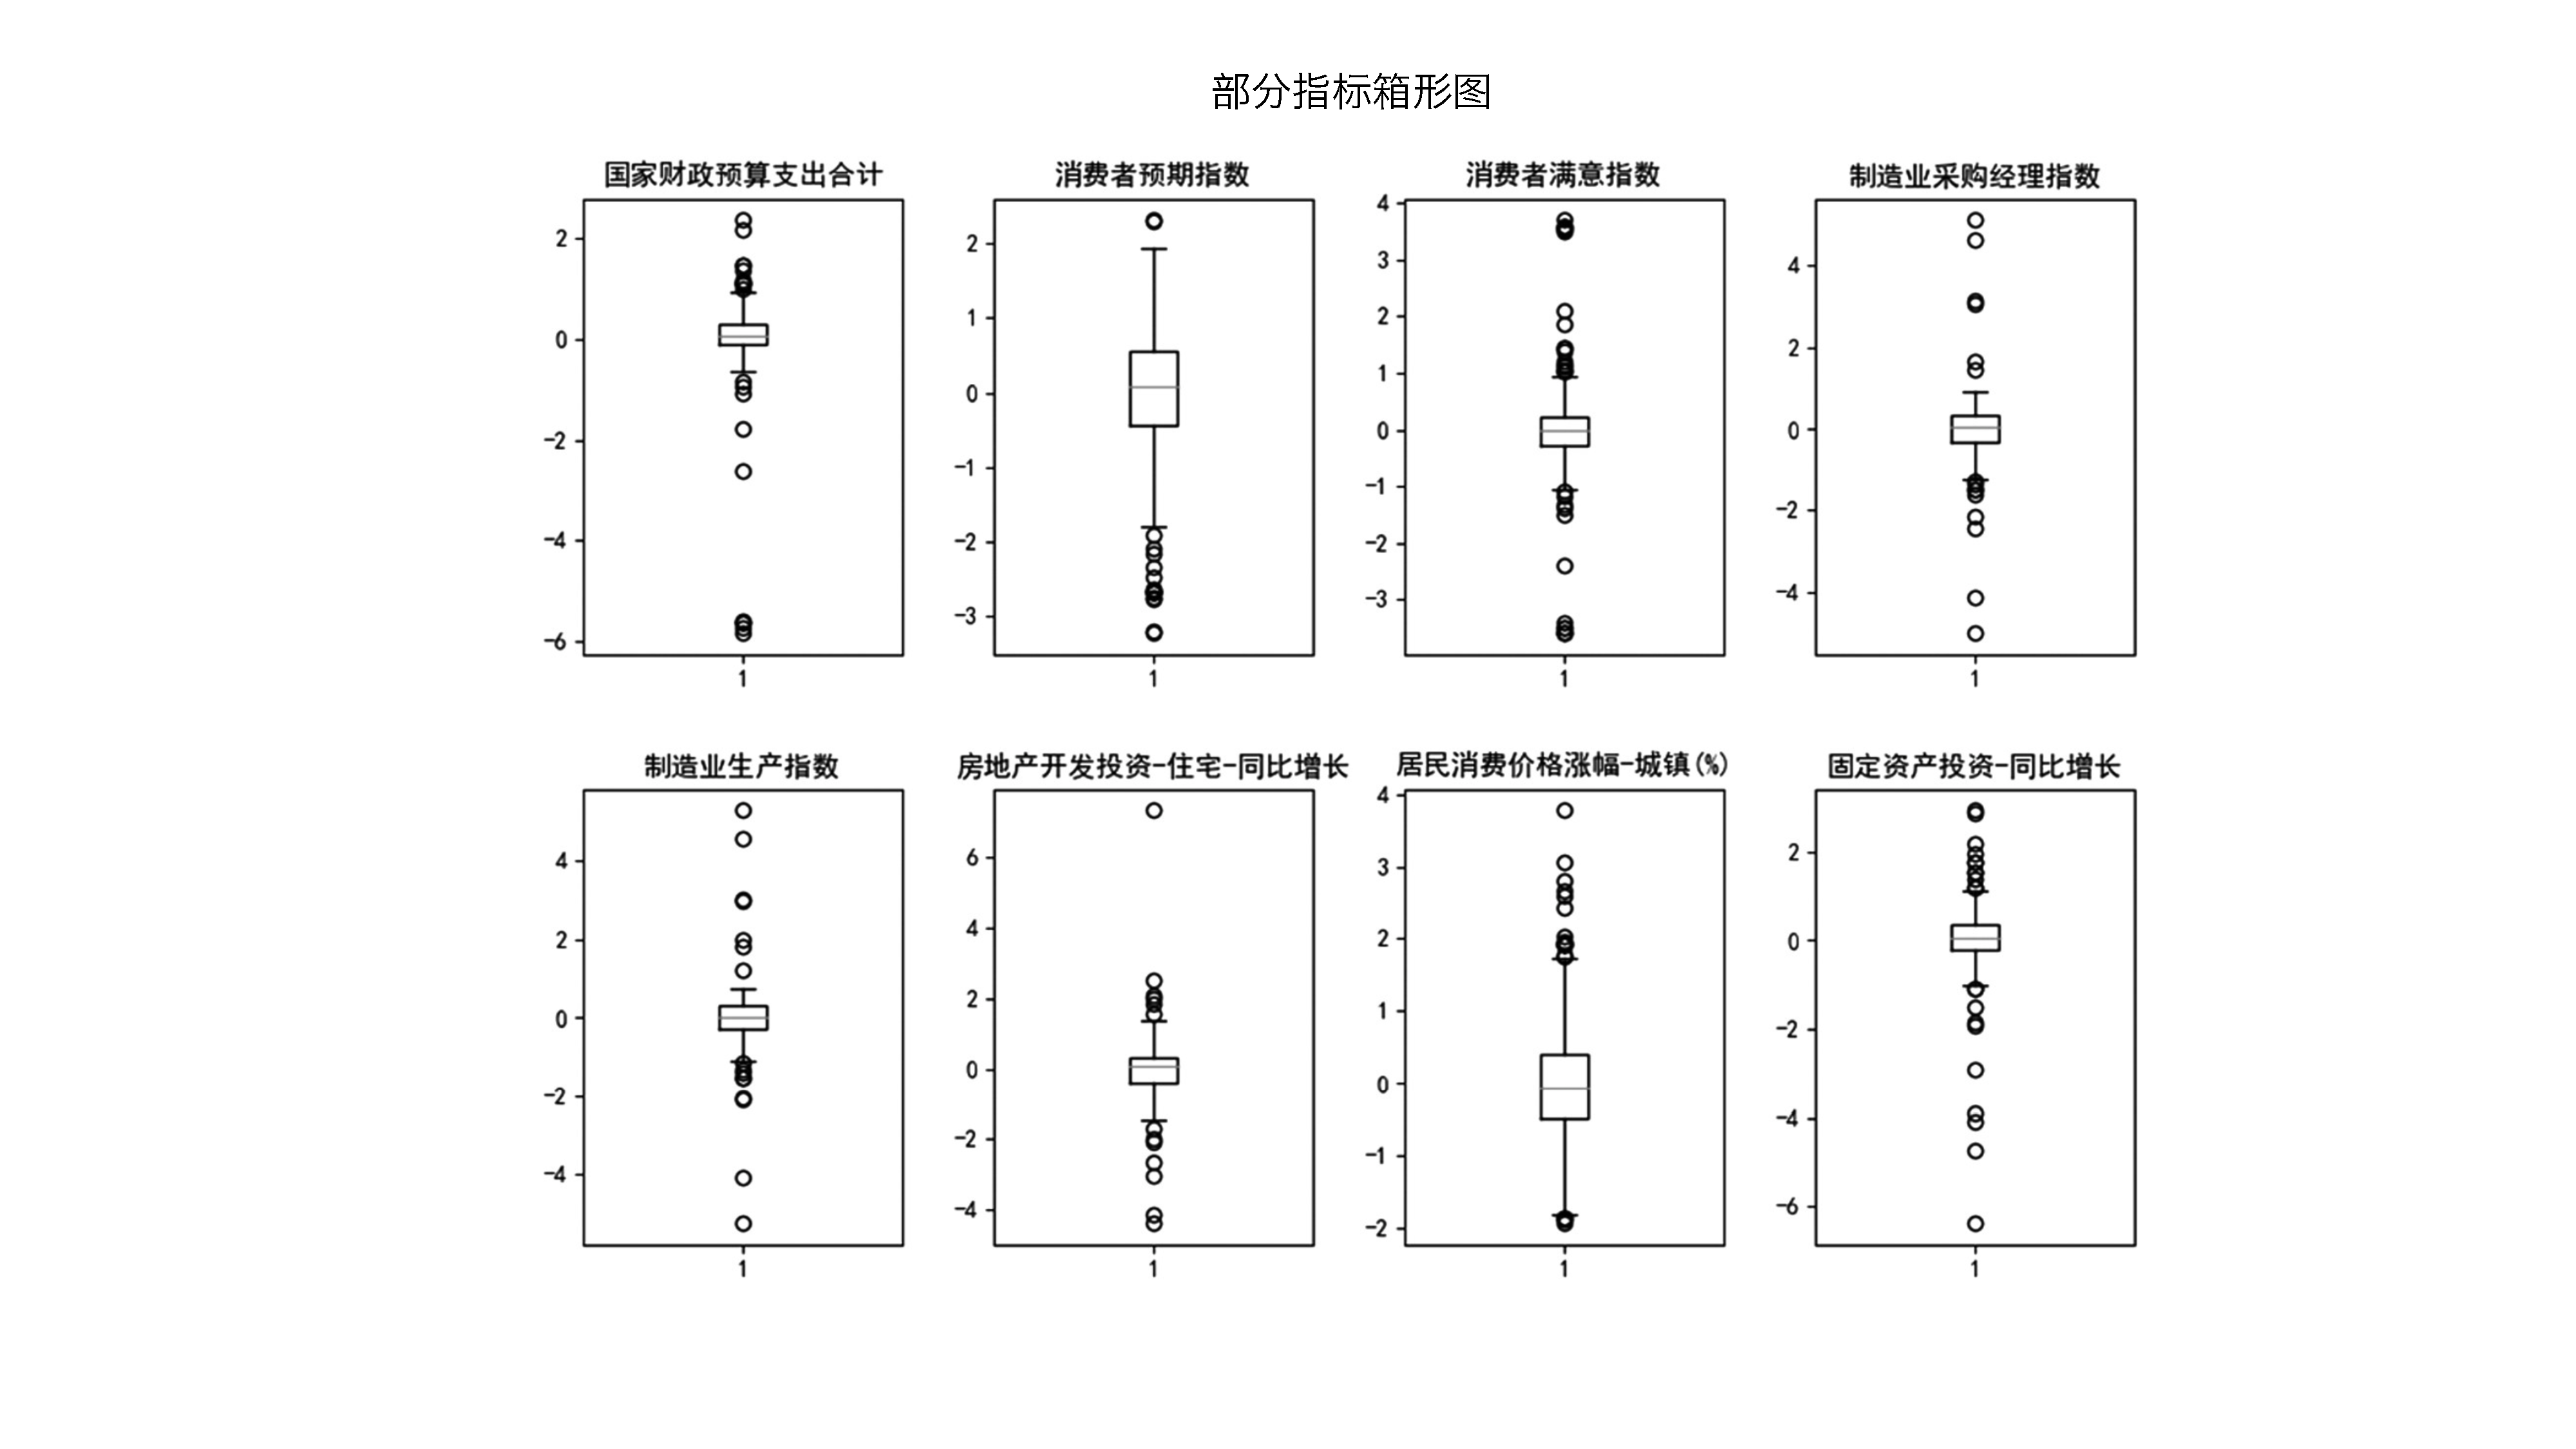
\includegraphics[width=18cm]{pics/chapter2/box.pdf}
    \end{minipage}
    \begin{minipage}[t]{1\textwidth}
    \centering
    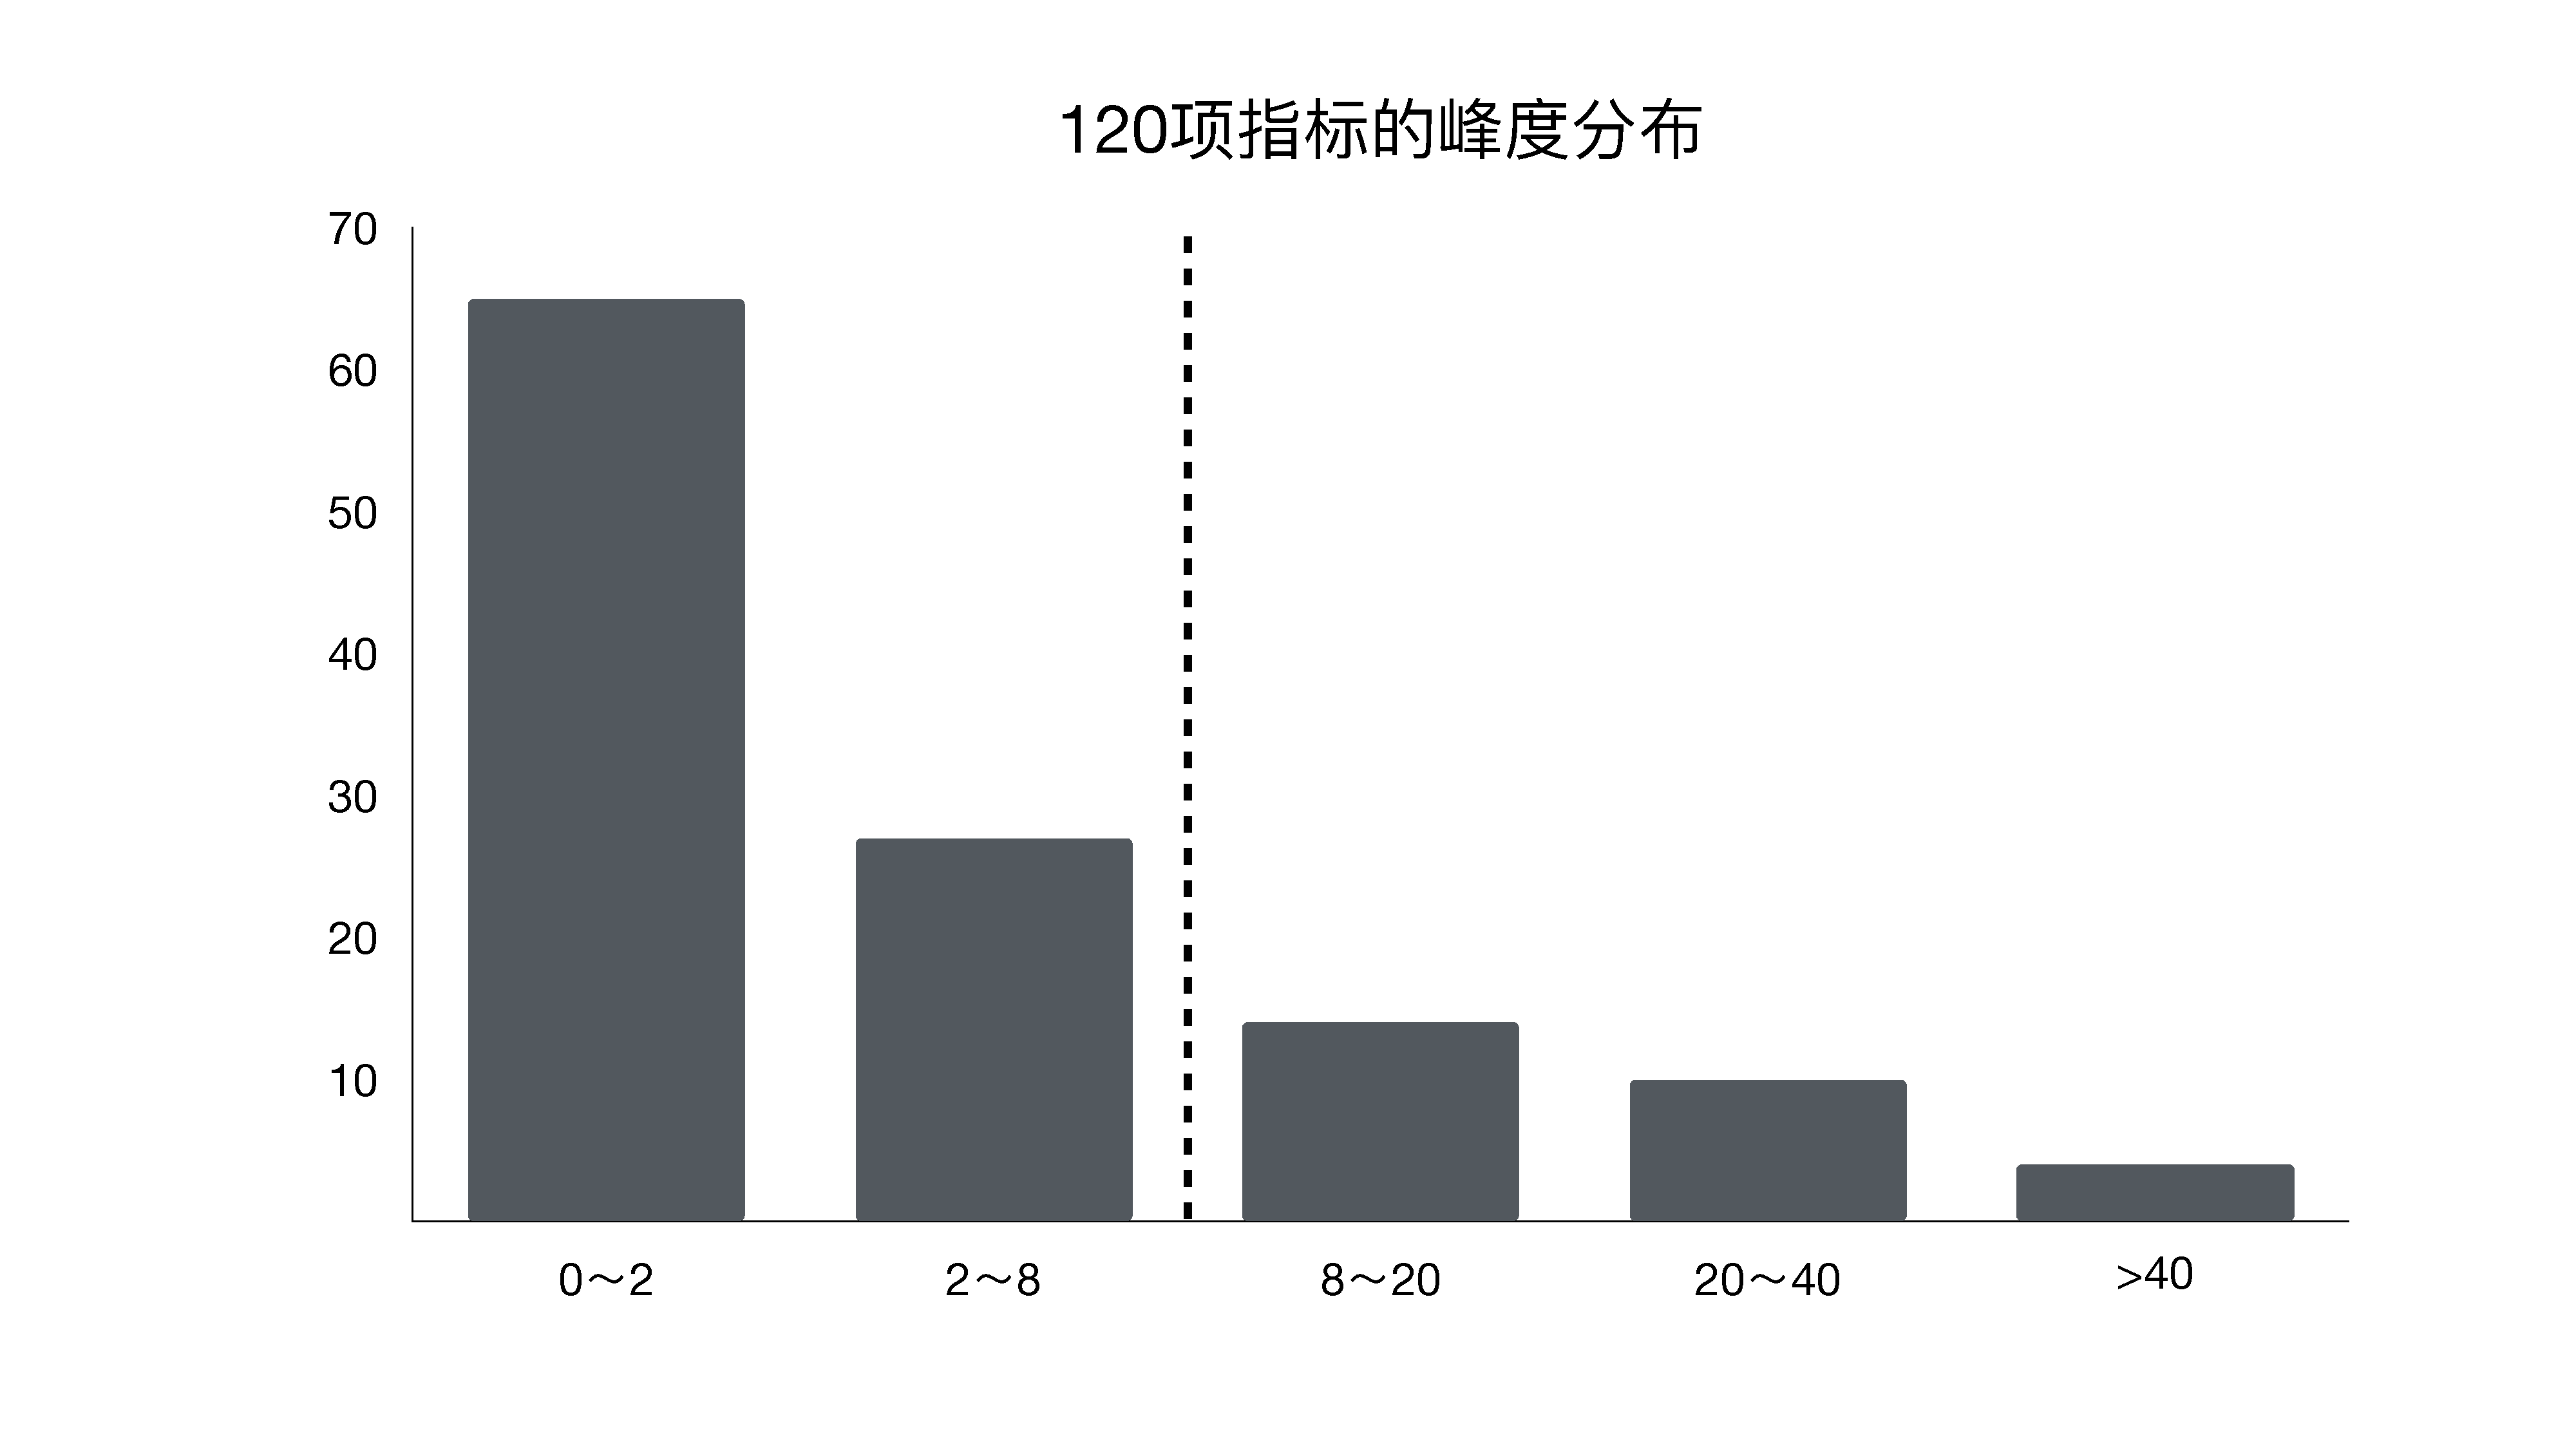
\includegraphics[width=12cm]{pics/chapter2/skew.pdf}
    \end{minipage}
    \caption{\small 部分指标的箱形图和各经济指标的峰度分布情况}
    \label{desc}
\end{figure}

由于某些指标曾多次改变统计口径、统计频率等原因,这些数据中包含许多的缺失数据。
另外,在1999~2019年这20年间,中国经济经历了许数次重大外部冲击,许多经济指标中含有大量离群值(见图\ref{desc}),
从各指标的经验分布的峰度值(一般峰度大于8就被认为是重尾,8是自由度为5的$t$分布的峰度值)来看,许多经济指标的分布存在分布重尾的现象。

在预处理阶段,我们对不平稳数据进行一阶差分;之后所有数据均进行标准化处理,我们不剔除任何离群值;
另外,对于缺失数据的情况,在进行$L_2$主成分分析时对原始数据进行插补,插补方法是对已有数据拟合ARMA模型
并根据估计得到的模型填补对应缺失数据。

下面介绍两组因子的主成分估计量的获得:首先进行$L_2$主成分分析并根据\eqref{number}选择最合适的因子个数
(本组数据得出最佳因子个数为8);接下来将$L_2$主成分估计的因子载荷矩阵作为交替凸优化算法$\bm{A}^0$的初始值,
然后求解得到$L_1$因子载荷。根据\eqref{factor}得出两组因子得分的估计:我们称为$L_1$因子和$L_2$因子。

\subsubsection{实证结果}

将得到的$L_1$因子和$L_2$因子看作$m$维随机向量的一组时间序列,根据\eqref{predict-factor-model}建立预测模型。
对预测结果的评价,下面选取了三种指标:MSE、MAE和MPAE,其计算方法如下($e_t$为$t$时期的预测误差)。
\begin{equation}
    \begin{array}{clr}
        \text{MSE} &= \frac{1}{n}\sum_{t=1}^n e_t^2 \\
        \text{MAE} &= \frac{1}{n}\sum_{t=1}^n |e_t| \\
        \text{MPAE} &= \frac{1}{n}\sum_{t=1}^n |e_t / y_t| \\
    \end{array}
\end{equation}

由于景气指数反映了经济中多方面特征,因此也可以将几种景气指数的时间序列作为预测变量,也根据\eqref{predict-factor-model}建立预测模型。
我们把$L_2$因子的三种平均误差指标作为基准,记录$L_1$的对应误差和它的比,作为对照我们这里将景气指数模型的预测情况也进行展示。
表\ref{outcome1}、表\ref{outcome2}和表\ref{outcome3}分别对应了$h = 1, 3, 6$,分别对应下一个月、下一个季度和半年后的预测情况。其中
IM为景气指数模型的预测情况;L1\ PCA为$L_1$因子的预测情况。表格中带有*号标记的变量名称表示对于该指标,使用$L_1$主成分估计的因子在三种预测误差
测度中有两种小于$L_2$主成分估计的因子。
\begin{table}[H]
    \centering

    \resizebox{\textwidth}{!}{
    \begin{tabular}{@{}ccccccc@{}}
    \toprule
                 & Rel MSE(L1 PCA) & Rel MSE(IM) & Rel MAE(L1 PCA) & Rel MAE(IM) & Rel MPAE(L1 PCA) & Rel MPAE(IM) \\ \midrule
    工业生产总值*     & 0.81            & 1.49        & 0.87            & 1.67        & 0.43             & 1.55         \\
    原油总产量* & 0.70            & 1.98        & 0.75            & 1.54        & 0.96             & 1.60         \\
    货币供应量M2*      & 0.76            & 1.25        & 0.90            & 1.19        & 0.45             & 0.97         \\
    固定资产投资总额*  & 0.89            & 1.03        & 0.97            & 0.99        & 0.81             & 1.32         \\
    房地产开发投资总额* & 0.79            & 0.98        & 0.95            & 1.00        & 0.91             & 1.20         \\
    社会消费品零售总额* & 0.84            & 1.25        & 0.87            & 1.12        & 0.45             & 1.17         \\
    出口总额    & 1.24            & 1.69        & 1.06            & 1.43        & 0.90             & 1.50         \\
    住宅新开工面积总数*  & 0.89            & 2.40        & 0.85            & 1.98        & 0.45             & 2.22         \\
    股票流通市值*      & 0.99            & 3.99        & 0.98            & 2.84        & 0.81             & 4.51         \\
    城乡储蓄存款余额*     & 0.93            & 1.01        & 0.98            & 0.99        & 0.98             & 1.56         \\ \bottomrule
    \end{tabular}
    }
    \caption{向前一个月预测结果}
    \label{outcome1}
\end{table}

\begin{table}[H]
    \centering
    \resizebox{\textwidth}{!}{
    \begin{tabular}{@{}ccccccc@{}}
    \toprule
                 & Rel MSE(L1 PCA) & Rel MSE(IM) & Rel MAE(L1 PCA) & Rel MAE(IM) & Rel MPAE(L1 PCA) & Rel MPAE(IM) \\ \midrule
                 工业生产总值*     & 0.85            & 1.16        & 0.95            & 1.22        & 1.32             & 1.93         \\
    原油总产量* & 0.98            & 1.39        & 0.97            & 1.20        & 0.93             & 1.12         \\
    货币供应量M2       & 1.08            & 1.20        & 1.05            & 1.44        & 0.66             & 1.70         \\
    固定资产投资总额*  & 0.99            & 1.11        & 0.98            & 1.28        & 0.82             & 0.89         \\
    房地产开发投资总额* & 0.91            & 0.94        & 0.92            & 1.12        & 0.66             & 0.99         \\
    社会消费品零售总额* & 0.62            & 1.12        & 0.85            & 0.99        & 1.26             & 1.05         \\
    出口总额    & 1.26            & 1.10        & 1.10            & 1.30        & 1.04             & 1.72         \\
    住宅新开工面积总数   & 0.81            & 1.62        & 1.12            & 1.78        & 1.04             & 1.23         \\
    股票流通市值   & 0.99            & 1.98        & 1.00            & 1.50        & 1.04             & 1.91         \\
    城乡储蓄存款余额*     & 0.99            & 1.35        & 0.96            & 1.02        & 0.94             & 1.17         \\ \bottomrule
    \end{tabular}
    }
    \caption{向前三个月预测结果}
    \label{outcome2}
\end{table}

\begin{table}[H]\label{outcome3}
    \centering
    \resizebox{\textwidth}{!}{
    \begin{tabular}{@{}ccccccc@{}}
    \toprule
                 & Rel MSE(L1 PCA) & Rel MSE(IM) & Rel MAE(L1 PCA) & Rel MAE(IM) & Rel MPAE(L1 PCA) & Rel MPAE(IM) \\ \midrule
                 工业生产总值*     & 0.91            & 1.20        & 0.93            & 1.12        & 0.68             & 1.81         \\
    原油总产量* & 1.00            & 1.30        & 0.94            & 1.18        & 0.79             & 1.77         \\
    货币供应量M2      & 0.84            & 1.12        & 1.06            & 1.05        & 1.46             & 1.08         \\
    固定资产投资总额*  & 0.88            & 1.43        & 0.94            & 1.29        & 0.93             & 1.85         \\
    房地产开发投资总额* & 0.90            & 1.01        & 0.91            & 1.12        & 0.73             & 1.07         \\
    社会消费品零售总额* & 0.64            & 1.39        & 0.79            & 1.20        & 1.30             & 1.34         \\
    出口总额   & 1.46            & 1.40        & 1.20            & 1.32        & 1.45             & 1.82         \\
    住宅新开工面积总数*  & 0.85            & 1.50        & 0.96            & 1.36        & 0.70             & 1.02         \\
    股票流通市值   & 0.98            & 2.24        & 1.01            & 1.96        & 1.28             & 2.98         \\
    城乡储蓄存款余额*     & 0.99            & 1.48        & 0.98            & 1.19        & 0.97             & 1.70         \\ \bottomrule
    \end{tabular}
    }
    \caption{向前六个月预测结果}
    \label{outcome3}
\end{table}

从结果中可以看出,$L_1$主成分估计的因子有着良好的预测表现。在对下一个月的预测中,其预测准确度略高于$L_2$主成分估计;
在对下一个季度和半年后的预测中,两者的表现类似。
通过和景气指数模型的对比来看,使用任何一种因子估计的预测总体表现都更准确,这也验证了Stock等人的结论\cite{stock2002forecasting}。
我们可以做出结论,$L_1$主成分分析同样可以用来作为近似因子模型的估计,并且应用于扩散指数模型进行宏观经济预测。这意味着
在处理数据有缺失、不满足高斯分布假设时,可以直接使用$L_1$主成分分析来估计因子模型,它不仅仅能提供更好的稳健性,
同时也拥有很好的预测效果。

\subsection{本章小结}
本章首先简要介绍了因子模型的基础理论,包括了正交因子模型、动态因子模型和近似因子模型的基本概念和模型参数的估计方法。
正交因子模型主要通过主成分分析法来估计,而动态因子模型估计较为困难,常常估计其静态形式。
我们介绍了近似因子模型的主成分估计,在这里是作为一种非参数估计,
而主成分估计得出的因子得分可以很好地应用于宏观经济预测。

基于以上事实,结合宏观经济数据的一些重尾和缺失特征,我们希望在进行主成分分析时作稳健性上的改进,故
提出了采用$L_1$范数的主成分分析代替$L_2$主成分分析来估计模型。我们对$L_1$主成分分析的问题进行了表述,介绍了
一种交替凸优化算法并给出其实现步骤,
并通过模拟实验论证了$L_1$主成分分析
的确具有更好的稳健性。

最后,为了验证$L_1$主成分分析能否代替$L_2$主成分分析作为近似因子模型的估计。我们基于国内的一组月度宏观经济数据作了实证
研究,将两种不同的主成分估计引用在扩散指数模型的预测上。实证研究的结果表明,因子模型的$L_1$主成分估计量同样适用于
进行宏观经济预测,具有良好的预测效果。这启发我们在处理宏观经济数据时,可以充分利用$L_1$主成分分析手段来加强
分析的稳健性。

$L_1$主成分分析在计算开销上大许多,我们介绍的交替凸优化算法在实证研究中也体现出来这一缺点。在本文后续研究中,
我们将对交替凸优化算法的改进做一些尝试。